\section{Contiki Overview}

\subsection{Network Overview}

\begin{figure}[H]
	\centering
	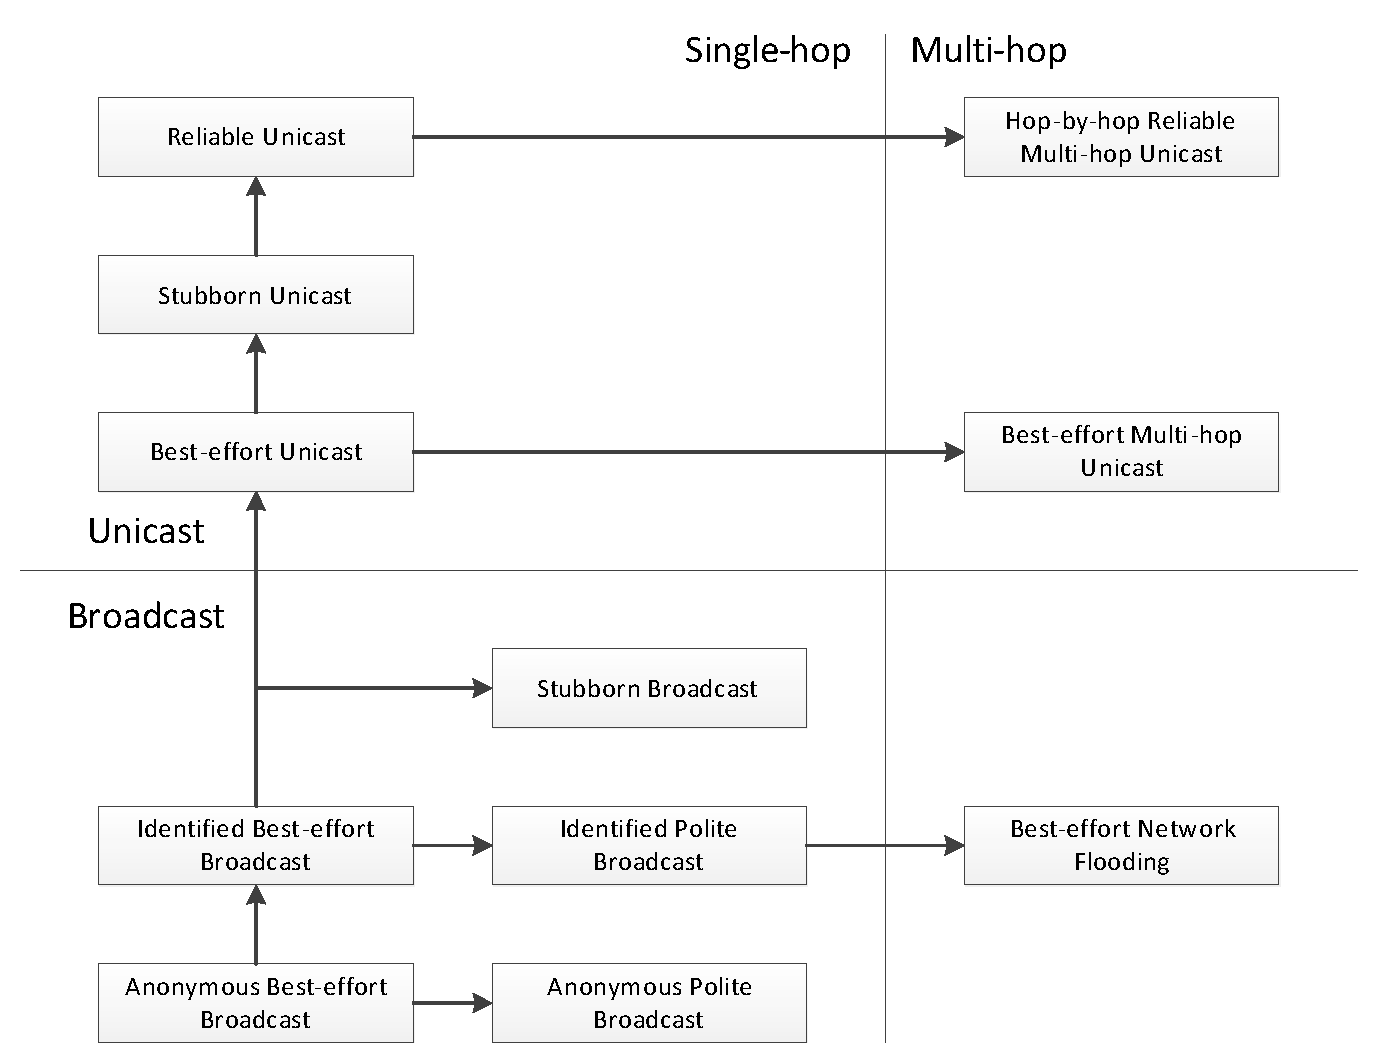
\includegraphics[width=\textwidth]{Diagrams/rime-stack}
	\caption{The communication primitives in the Rime network stack \cite{Dunkels:2007:ACA:1322263.1322295}}
\end{figure}

\begin{table}[H]
	\centering
	\begin{tabular}{ | l | l | l | }
		\hline
		Name & Header & Address \\
		\hline
		Anonymous Broadcast & abc.h & \url{contiki.sourceforge.net/docs/2.6/a01717.html} \\
		Broadcast & broadcast.h & \url{contiki.sourceforge.net/docs/2.6/a01720.html} \\
		Stubborn Broadcast & stbroadcast.h & \url{contiki.sourceforge.net/docs/2.6/a01739.html} \\
		Anonymous Polite Broadcast & polite.h & \url{contiki.sourceforge.net/docs/2.6/a01730.html} \\
		Polite Broadcast & ipolite.h & \url{contiki.sourceforge.net/docs/2.6/a01724.html} \\
		Unicast & unicast.h & \url{contiki.sourceforge.net/docs/2.6/a01738.html} \\
		Stubborn Unicast & stunicast.h & \url{contiki.sourceforge.net/docs/2.6/a01740.html} \\
		Reliable Unicast & runicast.h & \url{contiki.sourceforge.net/docs/2.6/a01738.html} \\
		Network Flooding (unreliable) & netflood.h & \url{contiki.sourceforge.net/docs/2.6/a01728.html} \\
		Network Flooding (reliable) & trickle.h & \url{contiki.sourceforge.net/docs/2.6/a01742.html} \\
		Multi-hop Unicast & mesh.h & \url{contiki.sourceforge.net/docs/2.6/a01725.html} \\
		Reliable Multi-hop Unicast & rmh.h & \url{contiki.sourceforge.net/docs/2.6/a01732.html} \\
		\hline
	\end{tabular}
	\caption{Communication Primitives headers and documentation location}
\end{table}

\begin{table}[H]
	\centering
	\begin{tabular}{ | l | l | l | l | }
		\hline
		Name & Reliable & Target & Sender Known\\
		\hline
		Anonymous Broadcast & No & 1-hop neighbours & No\\
		Broadcast & No & 1-hop neighbours & Yes\\
		Stubborn Broadcast & No & 1-hop neighbours & No\\
		Anonymous Polite Broadcast & No & 1-hop neighbours & No\\
		Polite Broadcast & No & 1-hop neighbours & Yes\\
		Unicast & No & destination & Yes\\
		Stubborn Unicast & No & destination & Yes\\
		Reliable Unicast & Yes & destination & Yes\\
		Network Flooding (unreliable) & No & network & ?\\
		Network Flooding (reliable) & Yes & network & ?\\
		Multi-hop Unicast & No & destination & ?\\
		Reliable Multi-hop Unicast & Yes & destination & ?\\
		\hline
	\end{tabular}
	\caption{Communication Primitives behaviour}
\end{table}

\subsubsection{Anonymous Broadcast}

\subsubsection{Broadcast}

\subsubsection{Stubborn Broadcast}

\subsubsection{Anonymous Polite Broadcast}

\subsubsection{Polite Broadcast}

\subsubsection{Unicast}

\subsubsection{Stubborn Unicast}

This is in fact anonymous, it will not send the address of the node that send the message in the header of the message. If a node needs to know who sent the message, then the sender's address should be included in the body.

\subsubsection{Reliable Unicast}

\subsubsection{Network Flooding}

\subsubsection{Multi-hop Unicast}

\subsubsection{Reliable Multi-hop Unicast}


\subsection{Network Channels}

Channels in Contiki are virtual \cite{tel-aviv-contiki-exercises}. This means that when a connection is opened if you do not want to receive packets from another connection then a different channel should be used. It does not mean that different radio frequencies are used. To use different radio frequencies the function \verb|cc2420_set_channel| should be used to change the frequency messages are broadcasted on.


\subsection{Timers}

\subsubsection{Event Timer}

\url{http://contiki.sourceforge.net/docs/2.6/a01667.html}

\subsubsection{Callback Timer}

\url{http://contiki.sourceforge.net/docs/2.6/a01666.html}
